\chapter{Plots gerados para a simulação antes do ajuste}\label{apdx:simantesantes}

\begin{figure}[H]
	\centering
	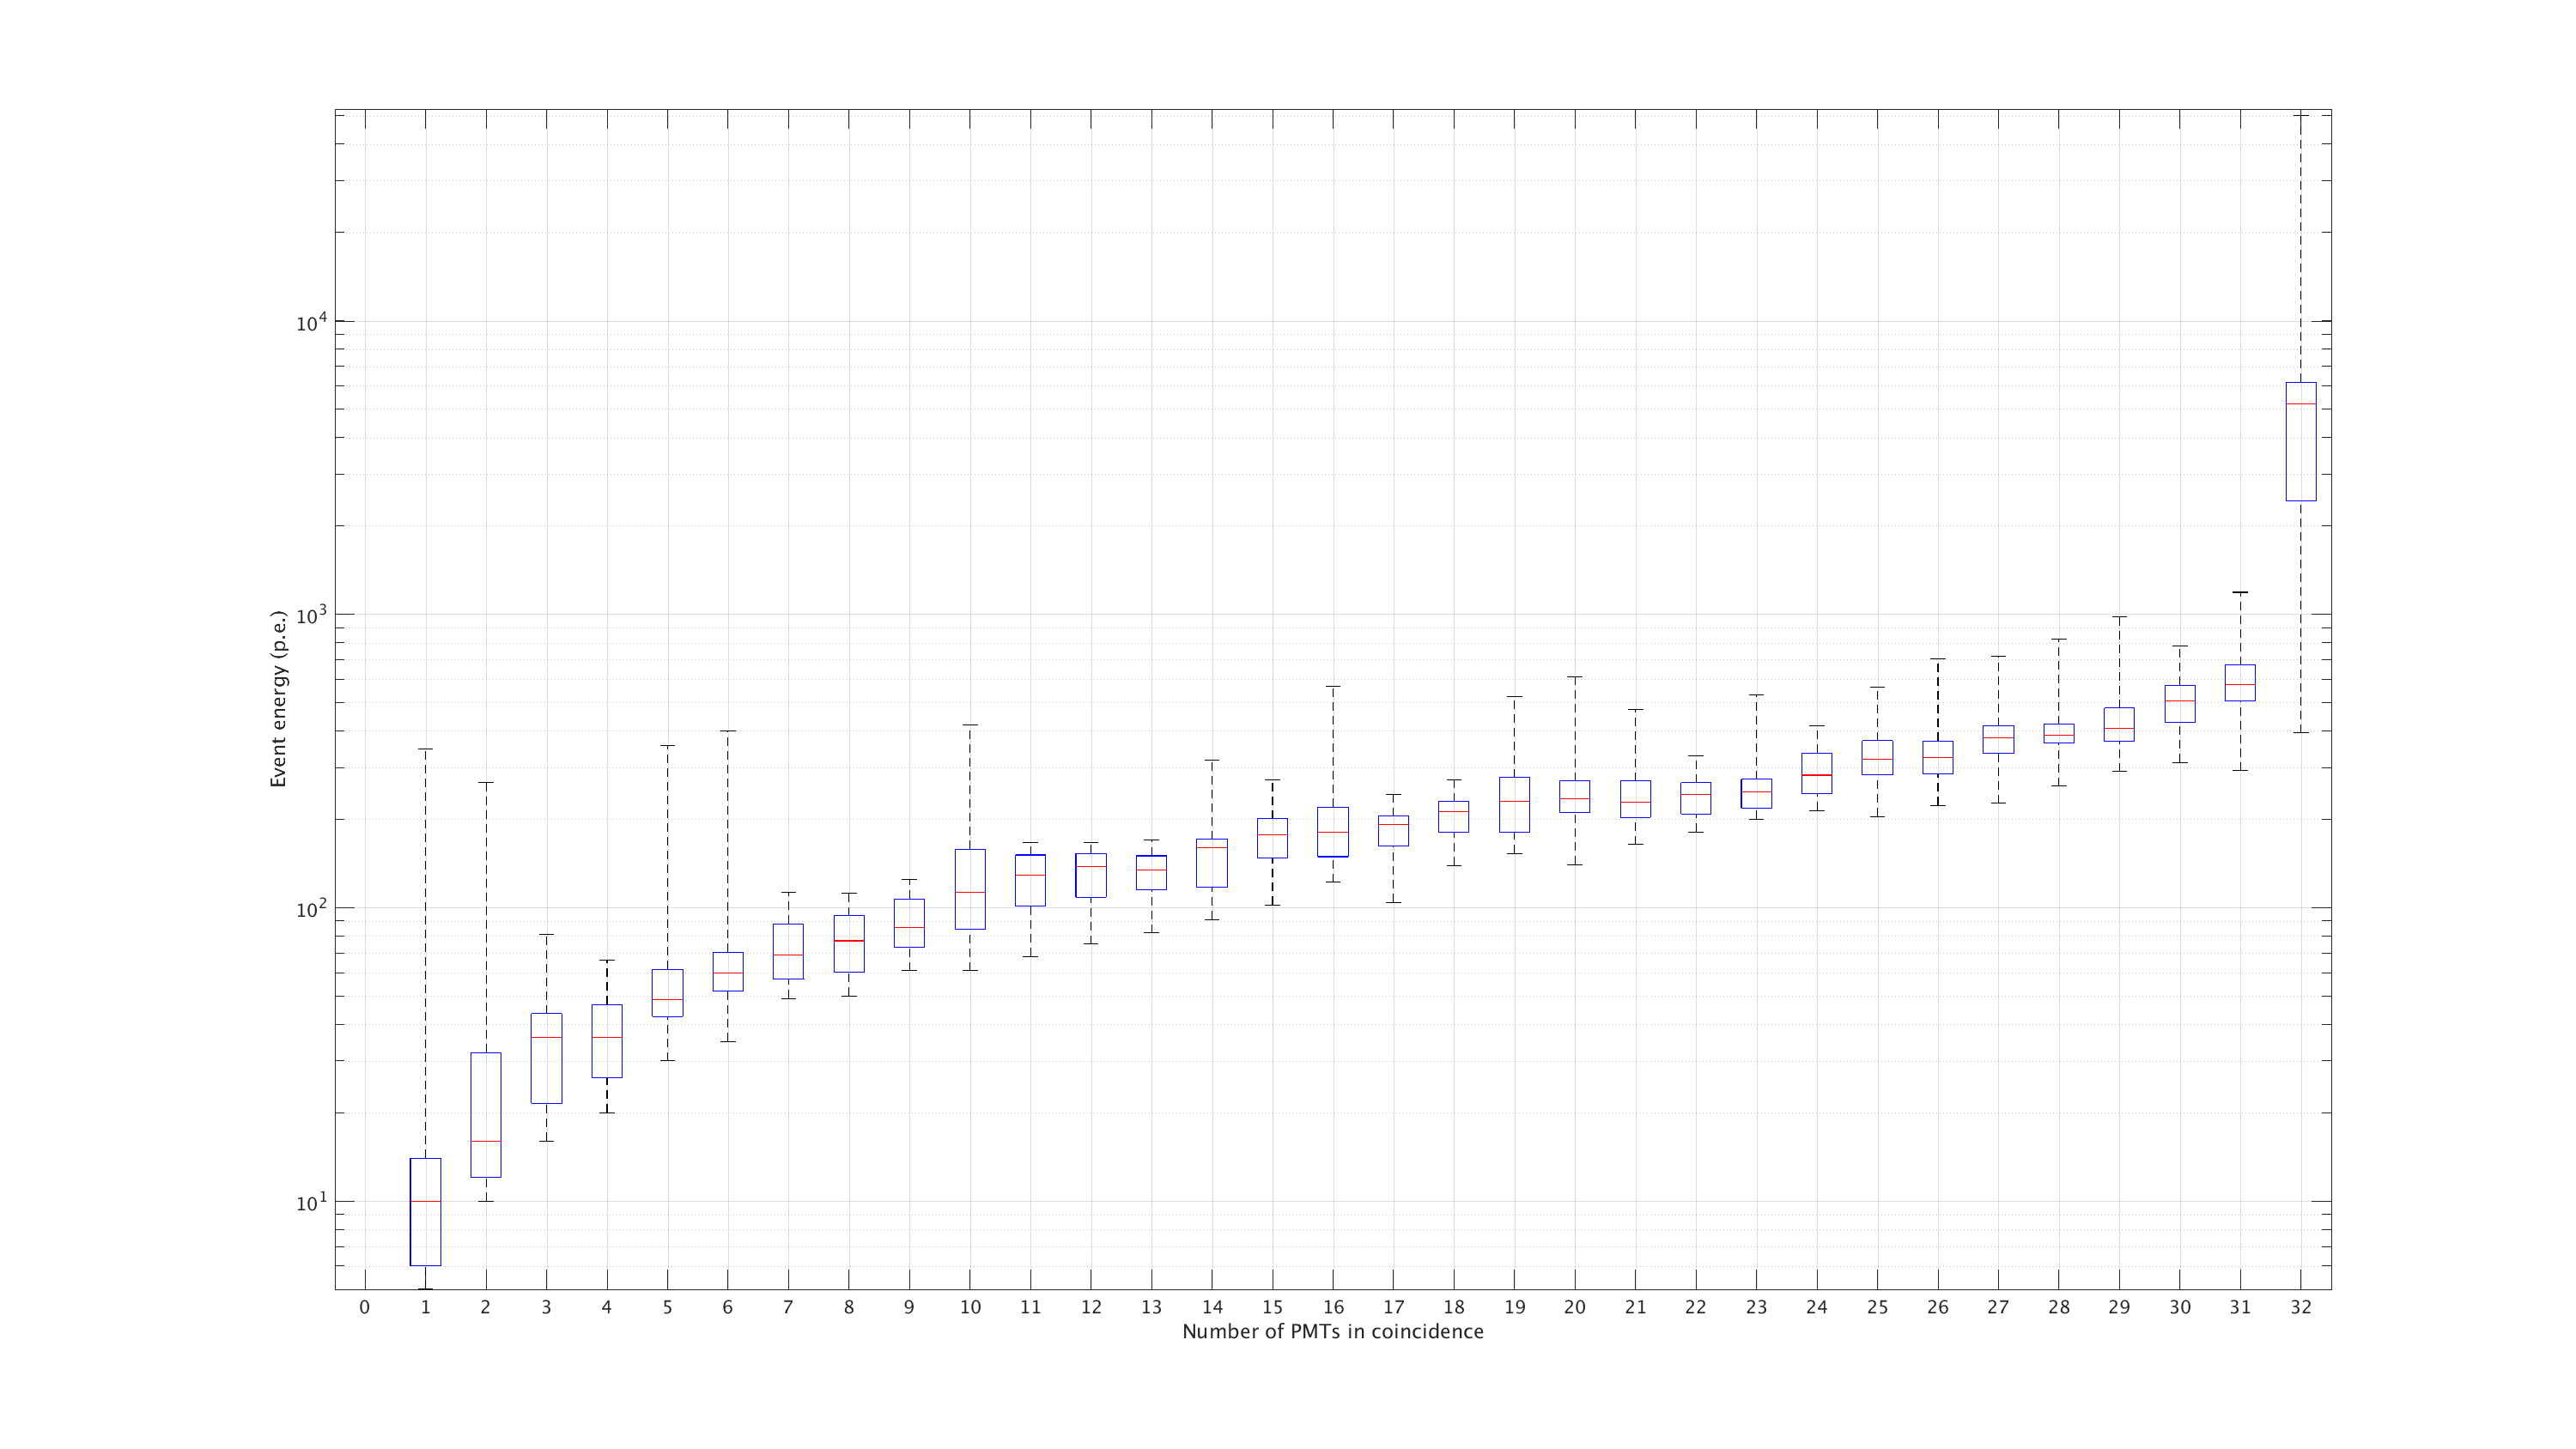
\includegraphics[width=16cm]{postextuais/apendice/simantes/boxplot.png}
	\caption{Distribuição de energia para eventos que dispararam exatamente n PMTs }
	\label{fig:transf}
\end{figure}

\begin{figure}[H]
	\centering
	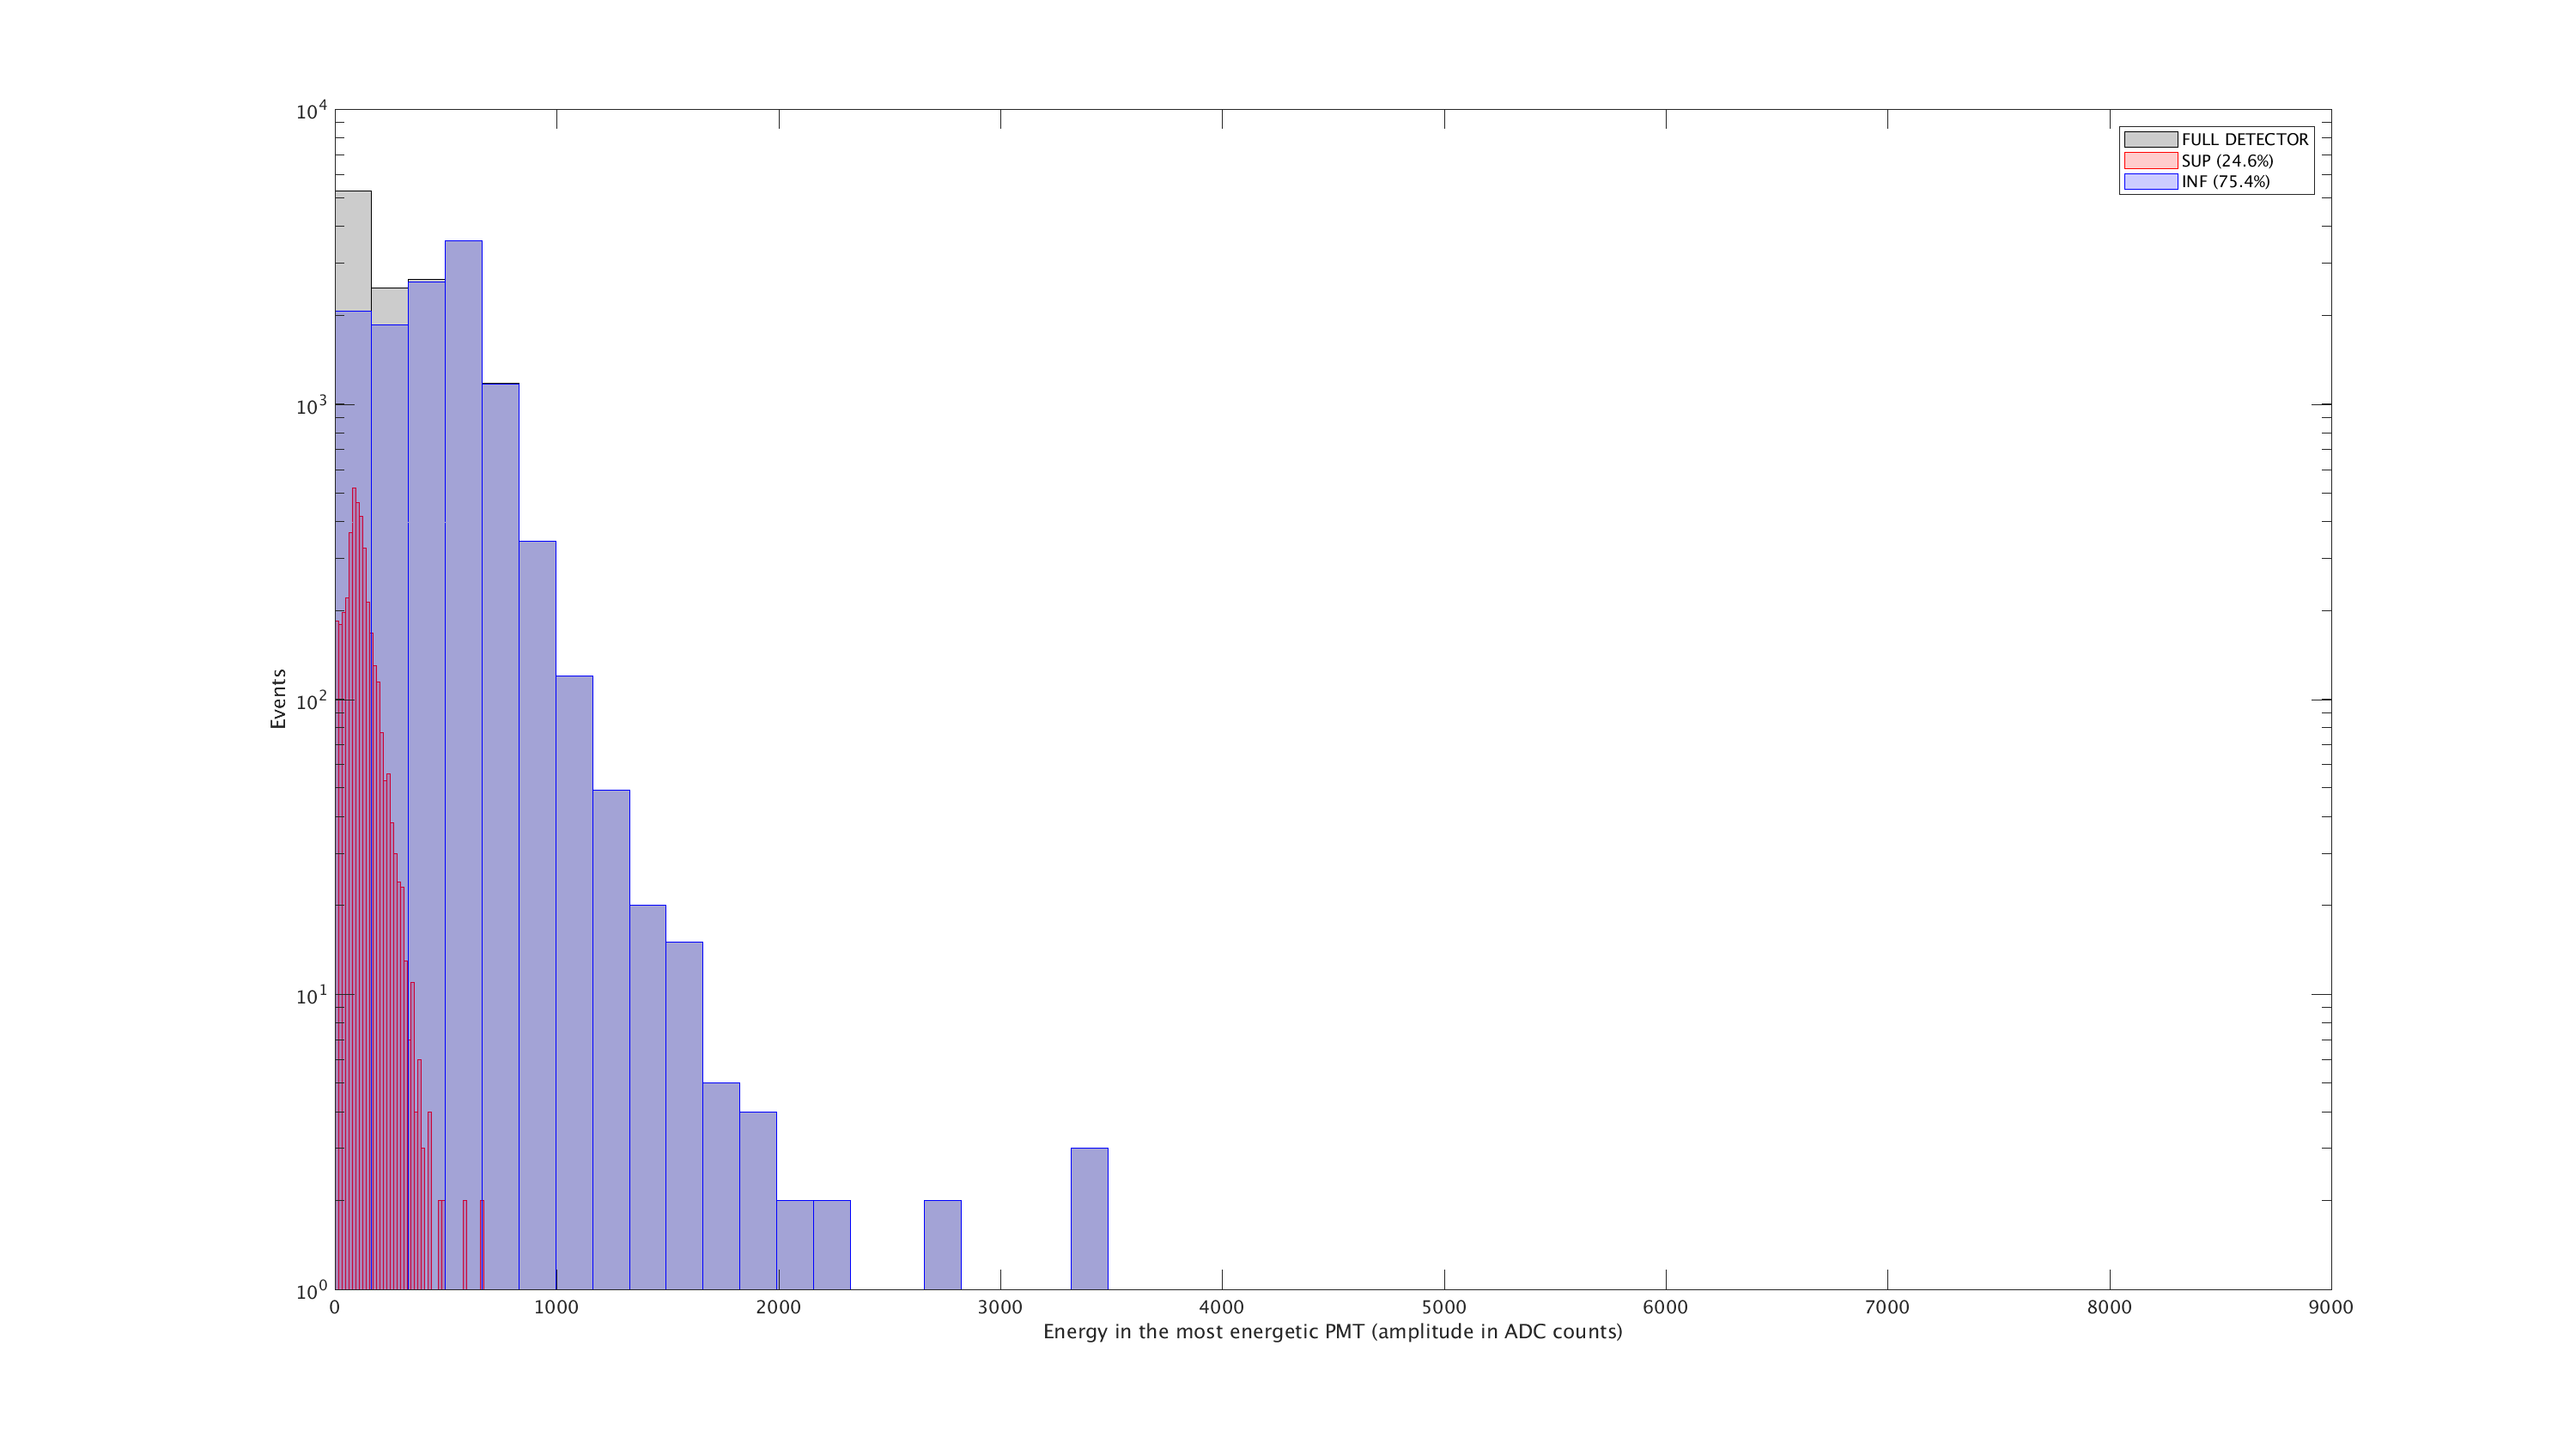
\includegraphics[width=16cm]{postextuais/apendice/simantes/energ_max_adc.png}
	\caption{Energia máxima em uma PMT por evento, separado em PMTs superiores e inferiores }
	\label{fig:transf}
\end{figure}

\begin{figure}[H]
	\centering
	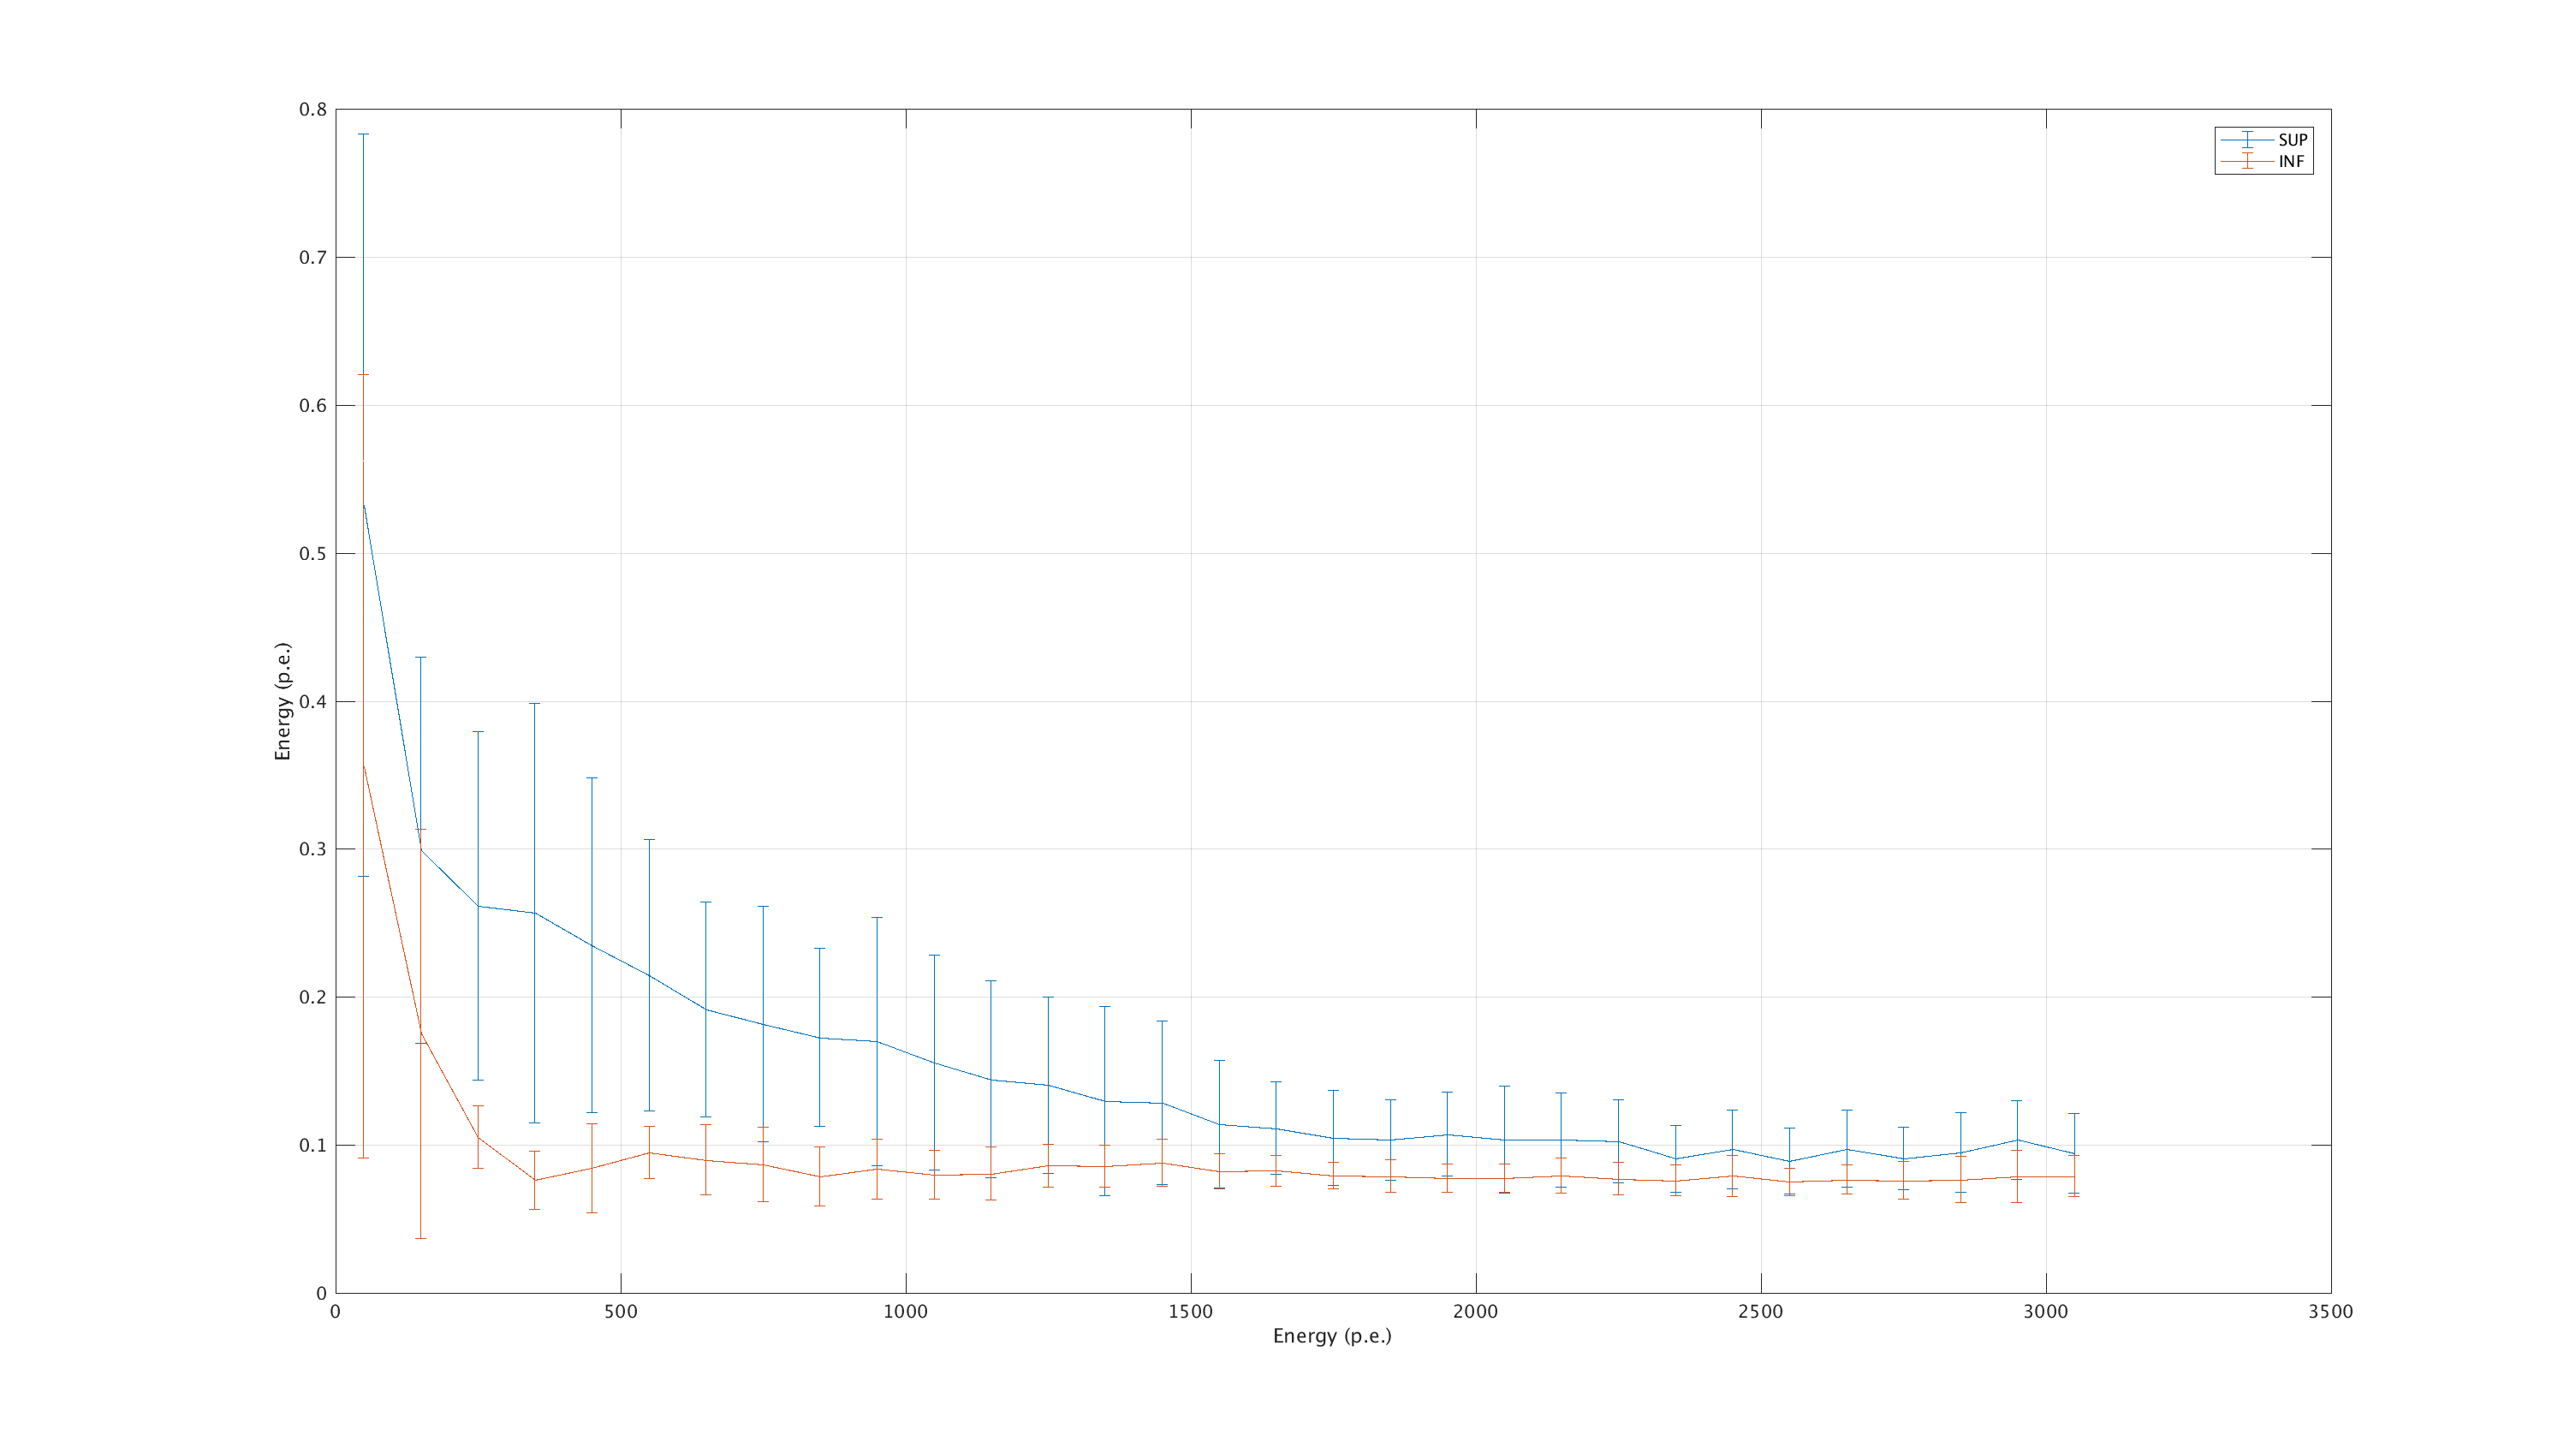
\includegraphics[width=16cm]{postextuais/apendice/simantes/errorbarene.png}
	\caption{Média e desvio padrão (representado pelas barras verticais) da percentagem de p.e. gerados na PMT mais energética pertencentes ao plano superior e inferior }
	\label{fig:transf}
\end{figure}

\begin{figure}[H]
	\centering
	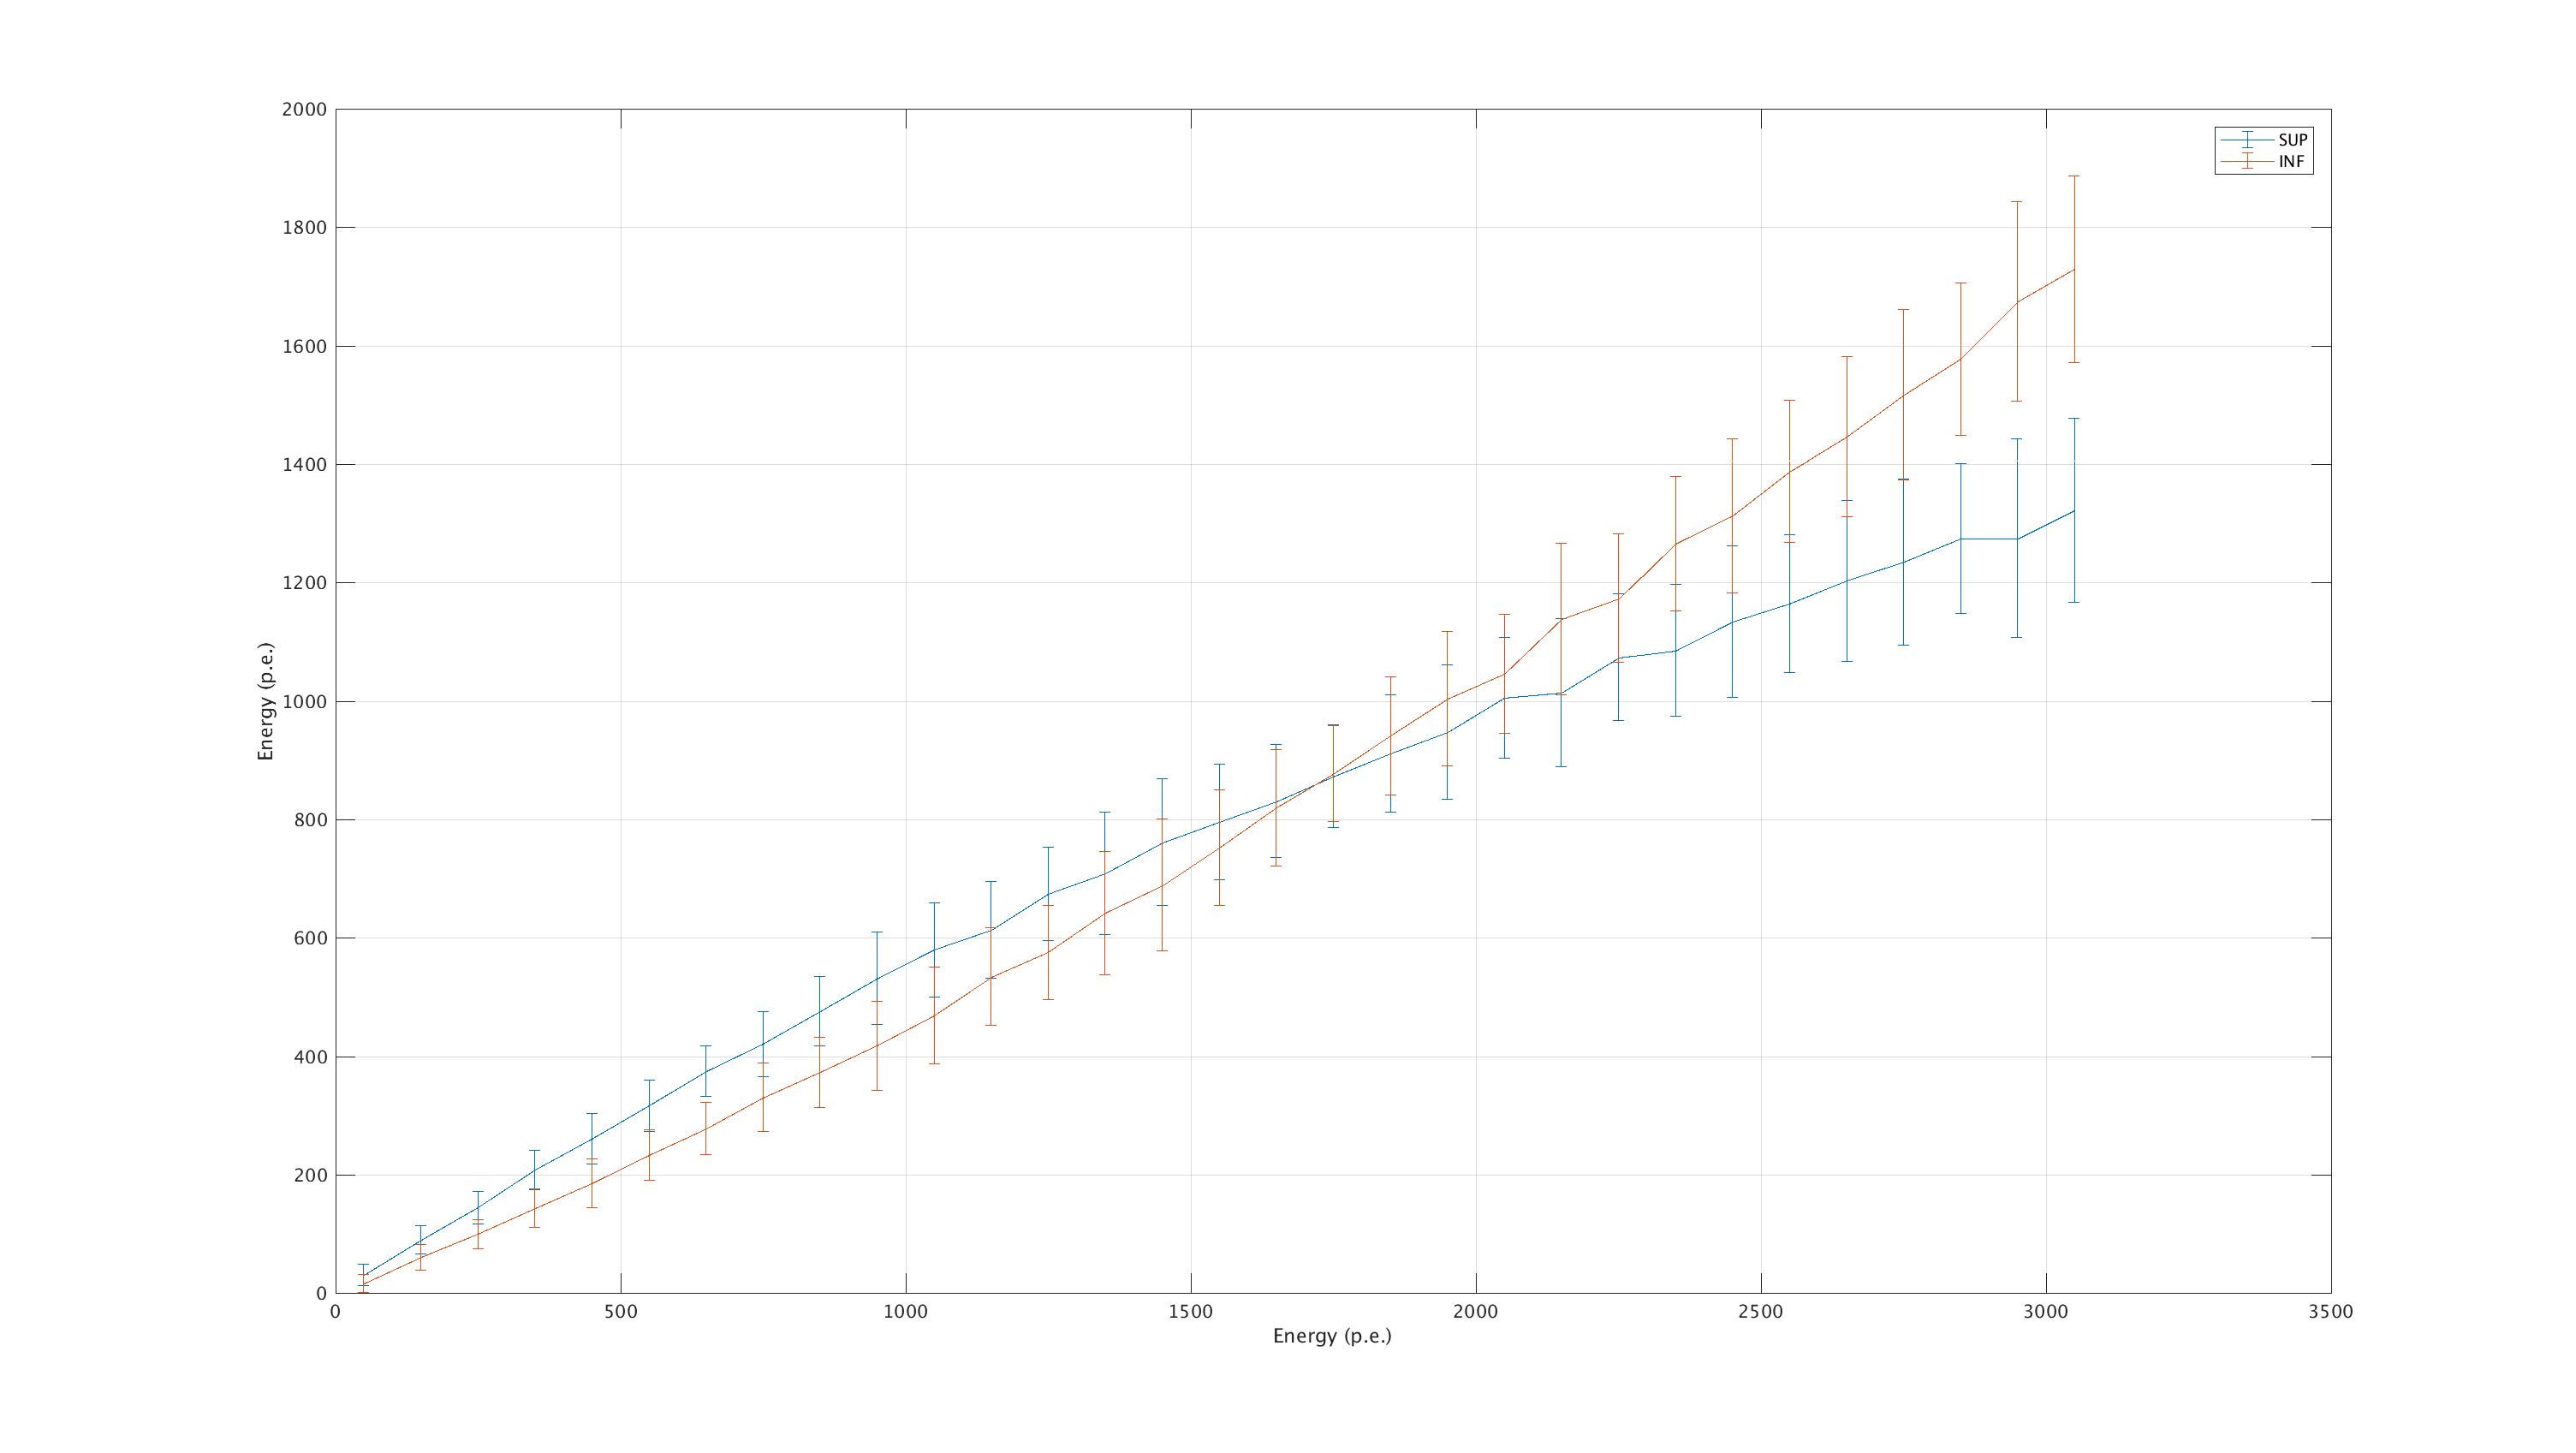
\includegraphics[width=16cm]{postextuais/apendice/simantes/errorbarmosten.png}
	\caption{Média e desvio padrão das distribuições de energia por evento nas PMTs superiores e inferiores }
	\label{fig:transf}
\end{figure}

\begin{figure}[H]
	\centering
	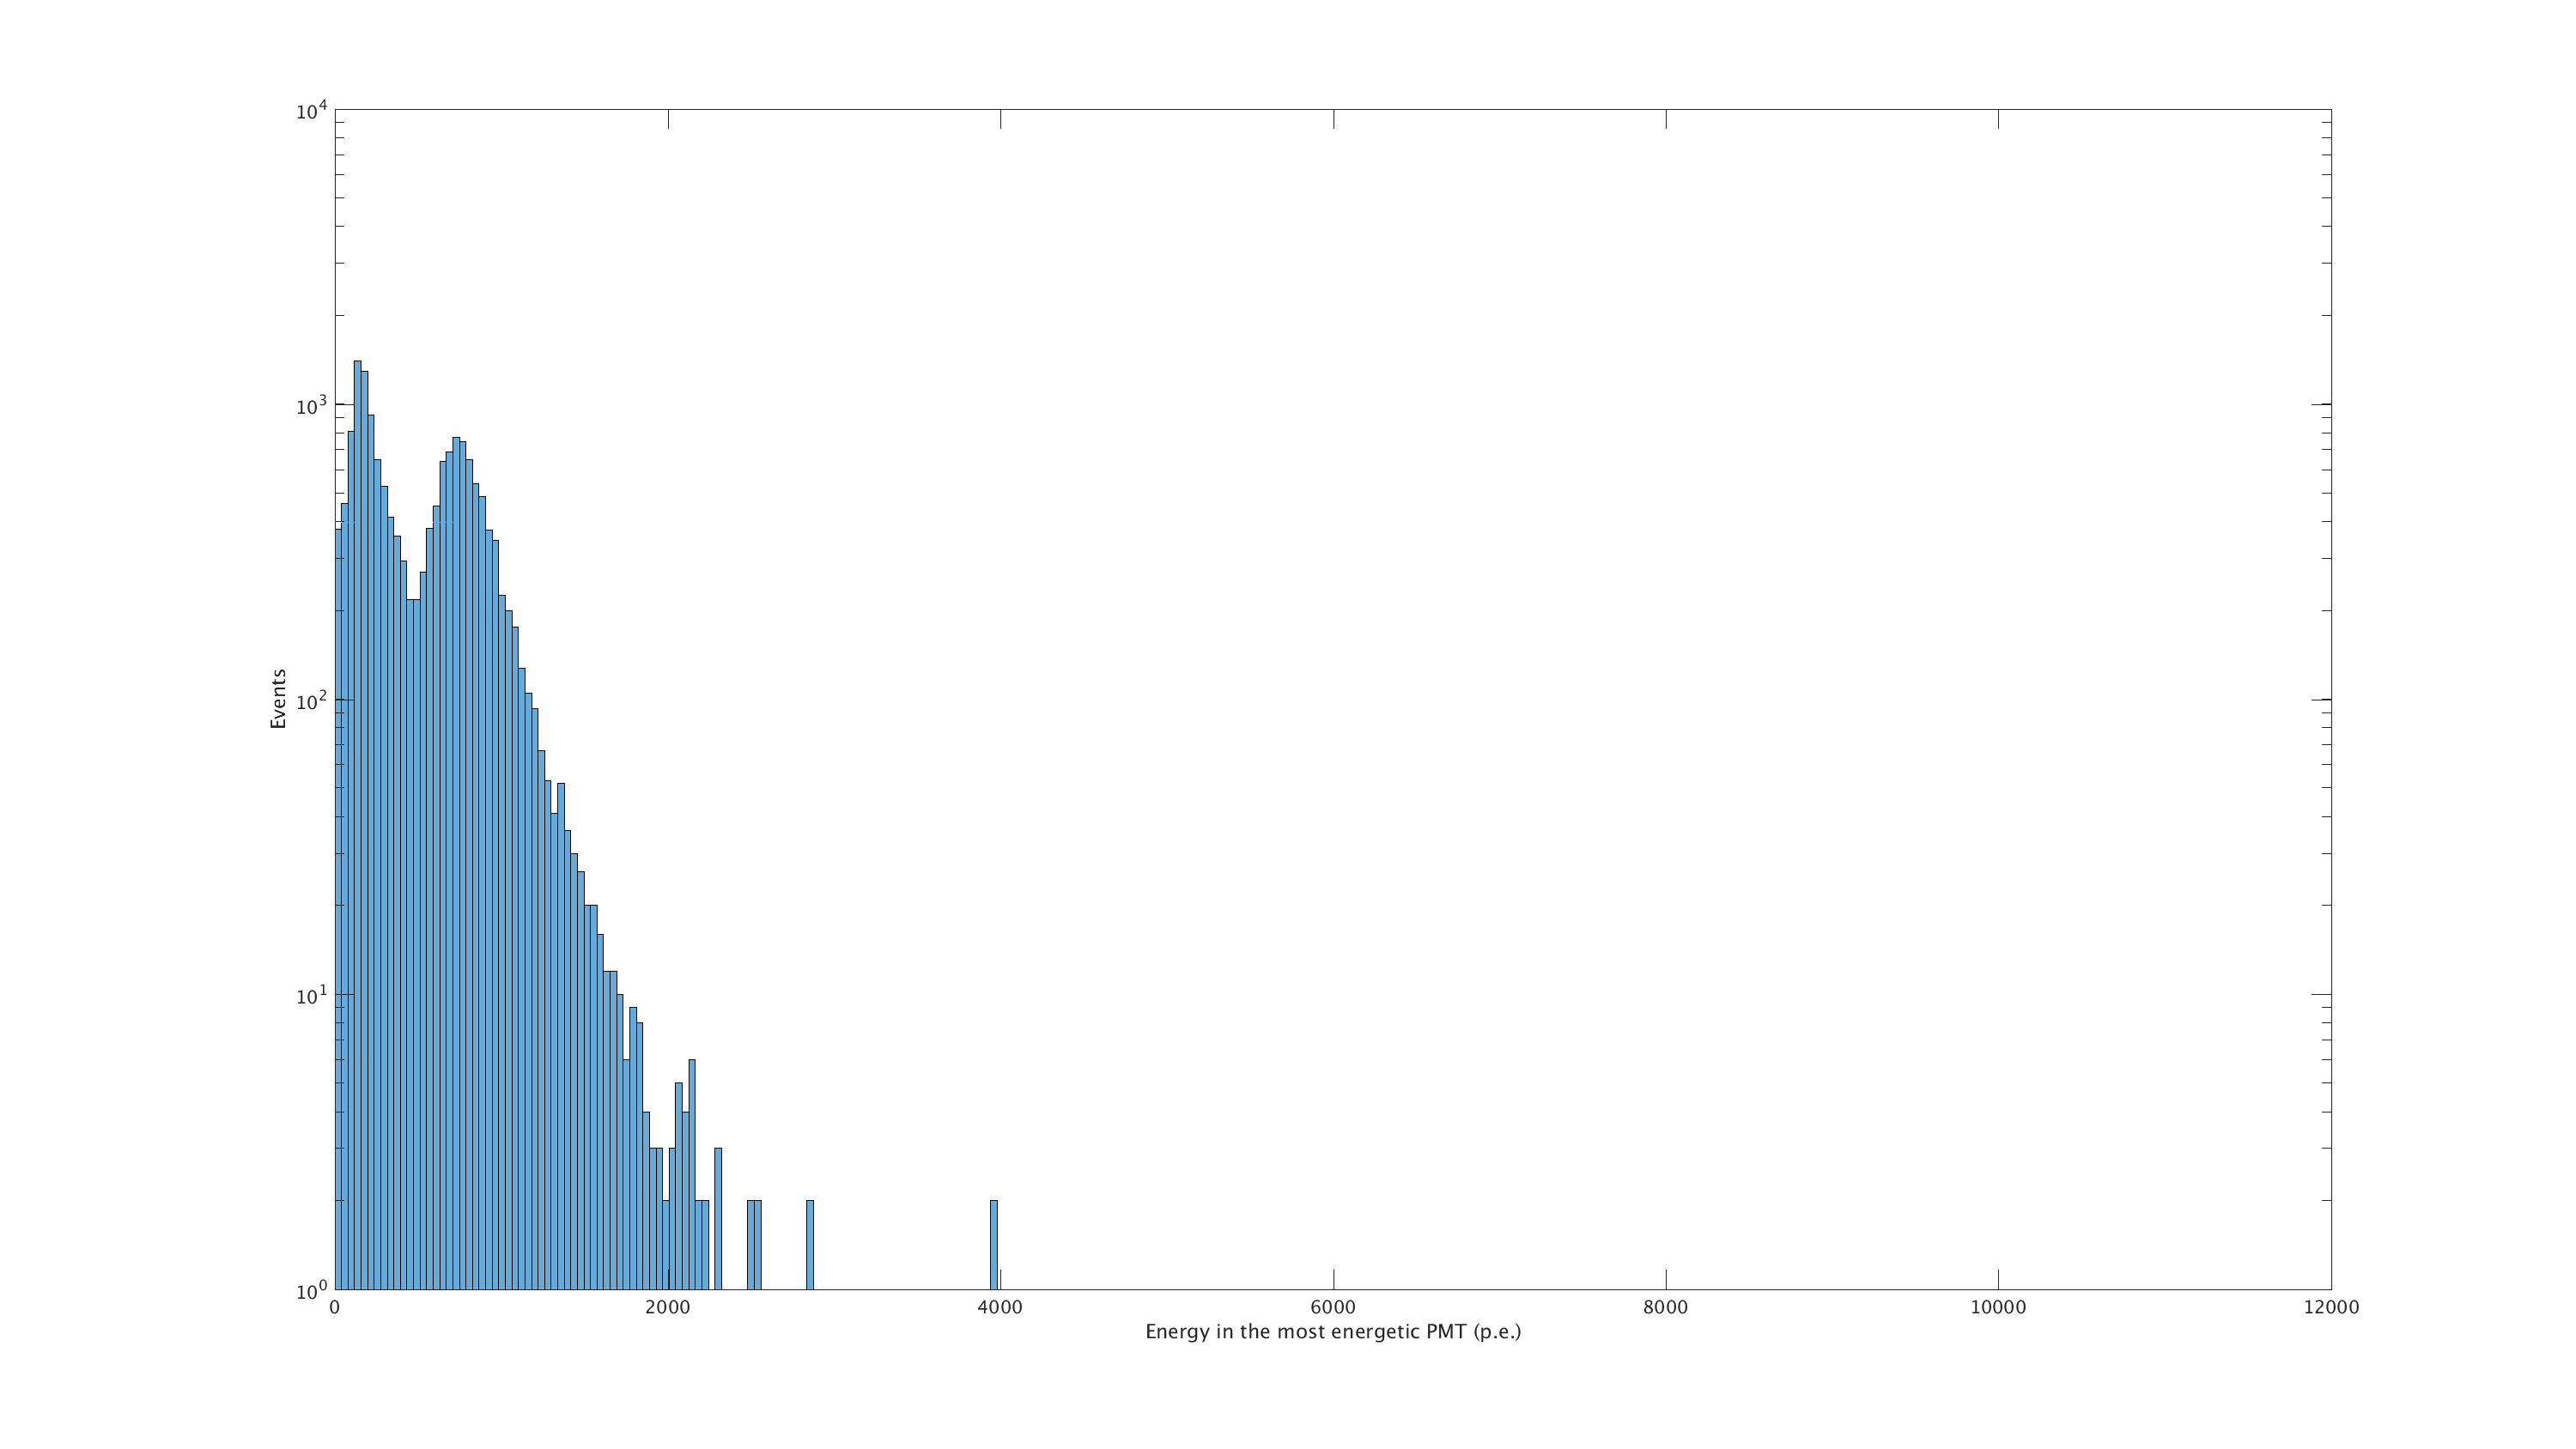
\includegraphics[width=16cm]{postextuais/apendice/simantes/mosten_pmt.png}
	\caption{Energia máxima de uma PMT por evento, em p.e. }
	\label{fig:transf}
\end{figure}

\begin{figure}[H]
	\centering
	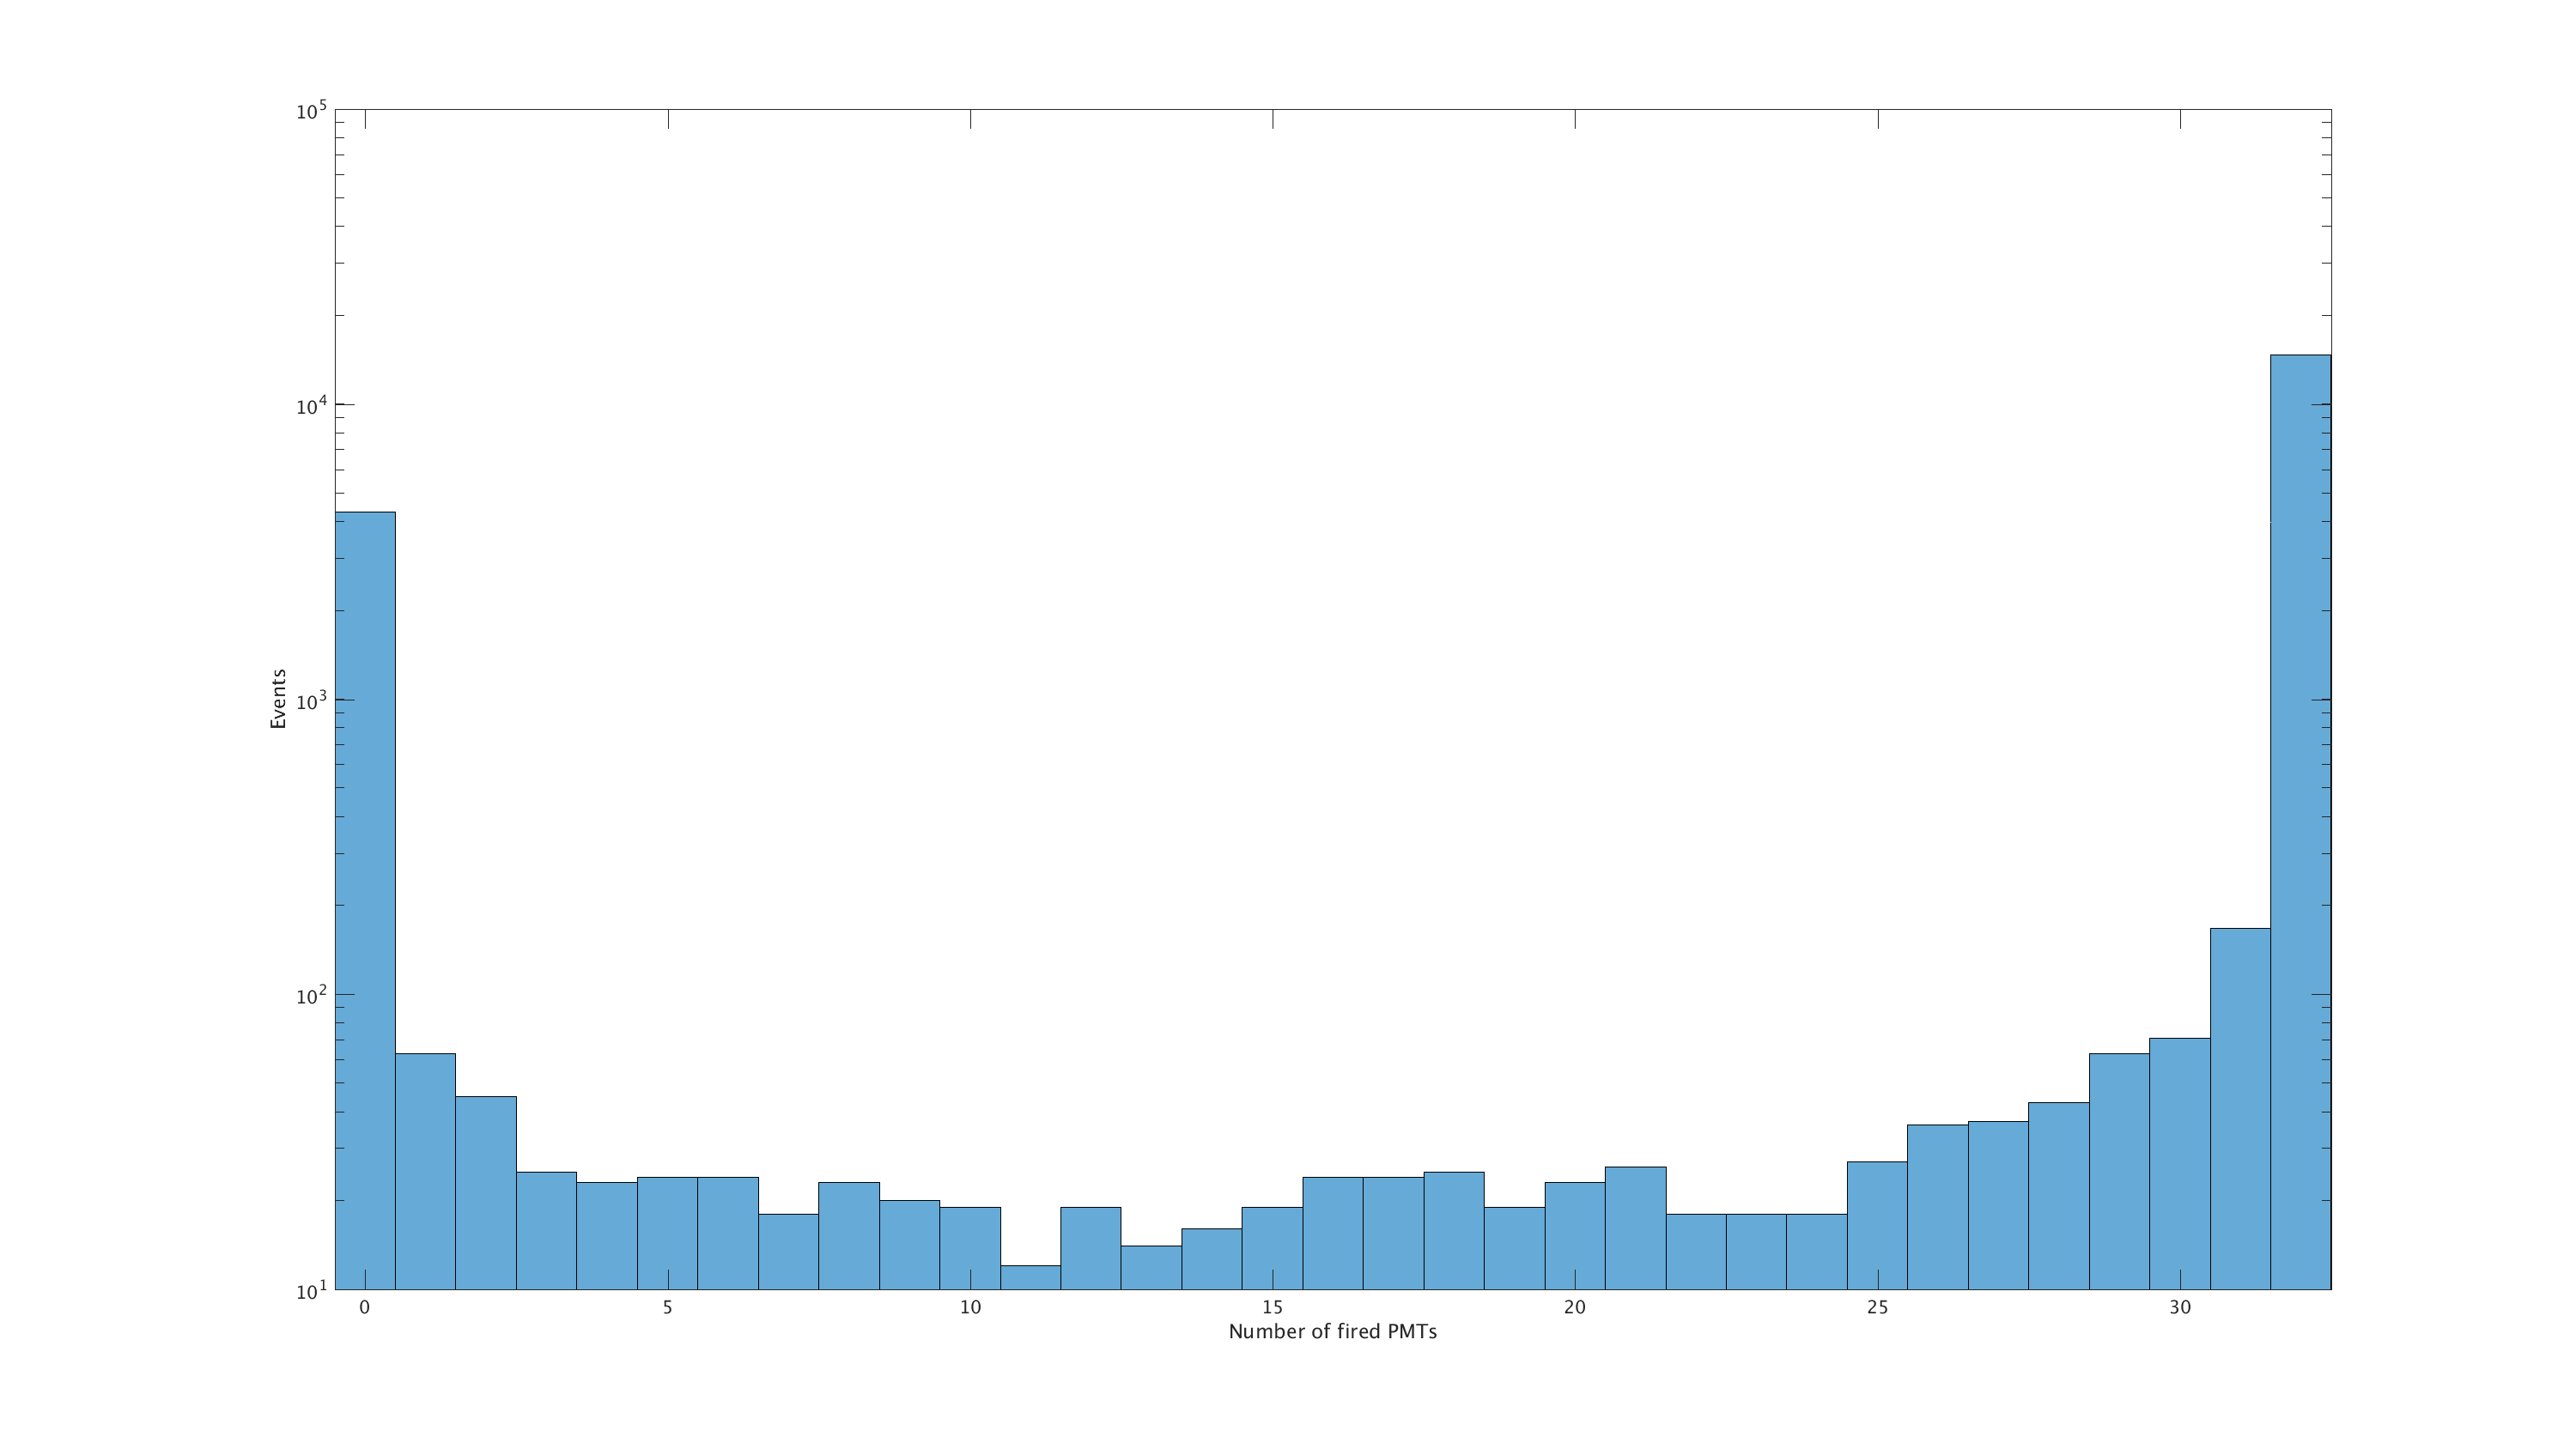
\includegraphics[width=16cm]{postextuais/apendice/simantes/firedpmt.png}
	\caption{Histograma de PMTs disparadas por evento}
	\label{fig:transf}
\end{figure}

\begin{figure}[H]
	\centering
	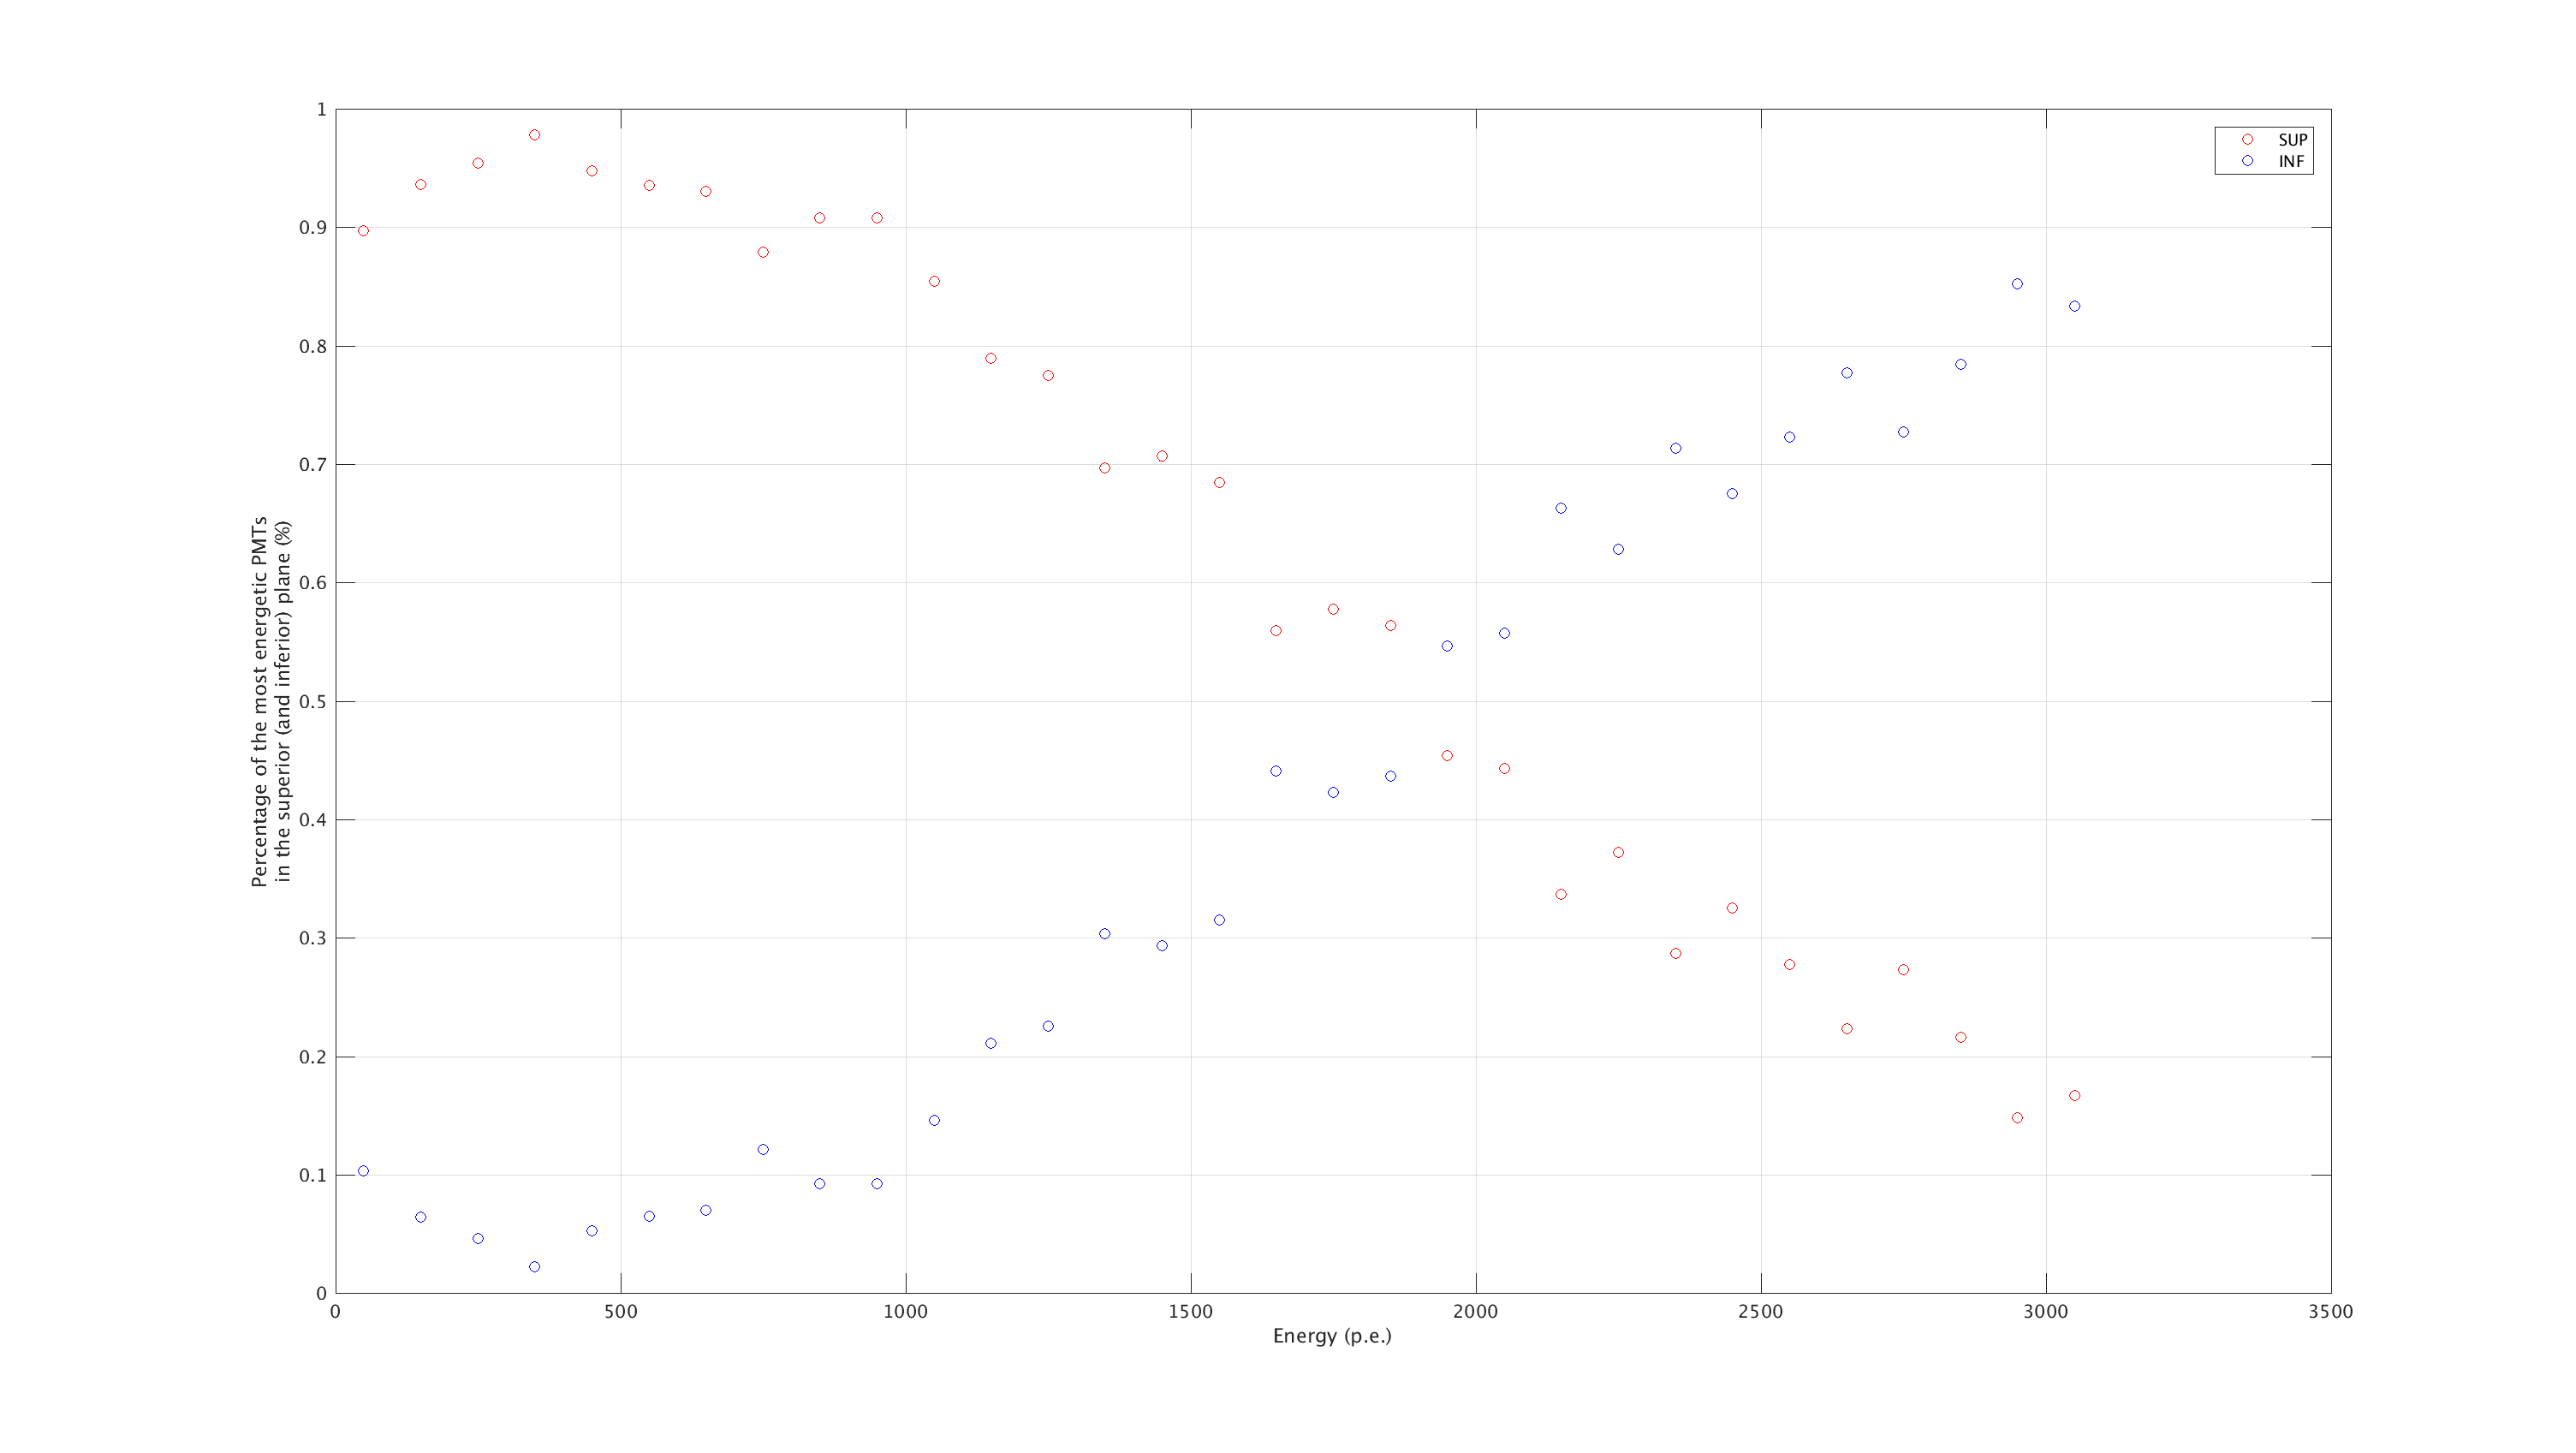
\includegraphics[width=16cm]{postextuais/apendice/simantes/probsupinf.png}
	\caption{Probabilidade da posição mais energética para PMTs superiores e inferiores}
	\label{fig:transf}
\end{figure}